%----------------------------------------------------------------
%
%  File    :  chapter3.tex
%
%  Authors :  Keith Andrews, IICM, TU Graz, Austria
%             Manuel Koschuch, FH Campus Wien, Austria
% 
%  Created :  22 Feb 96
% 
%  Changed :  30 Oct 2008
%  !TEX root = ./thesis.tex
%----------------------------------------------------------------


\chapter{Design Entwicklung der MCKB Applikation}
\label{chap:xamarinformsdevelopment}

	Als Basis für diese Arbeit dienen zwei während des Studiums entwickelte mobile Applikationen.
	\begin{enumerate}
		\setlength\itemsep{0em}
		\item \textbf{STM32KB}\footnote{Download via http://m4xwe11o.ddns.net/MAD-Test/App/stm32kb.apk} - Mit Android Studio, in JAVA, entwickelte Applikation im 4. Semester an der FH Campus Wien
		\item \textbf{STM32CP} - Mit Visual Studio for Mac, in C\#, entwickelte Cross-Plattform Variante im 5. Semester an der FH Campus Wien
	\end{enumerate}
	Erstere Applikation wurde im Zuge der \textbf{Mobile App Development (MAD)} Vorlesung, zur Vertiefung von Software Engineering Skils unter Android Studio in JAVA entwickelt. Diese App ermöglicht die Darstellung von Artikeln zur Programmierung eines Mikrocontroller $\mu$C der Firma STM, um häufige Fragen zur Konfiguration unterschiedlicher Funktionen wie zum Beispiel \textit{UART (Universal Asynchronous Receive and Transmit)}, \textit{ADC (Analogue Digital Converter)} oder \textit{CAN (Controller Area Network)} einfach erklärt nachzulesen. Die App selber stellt nur die in einer MySQL Datenbank gespeicherten Artikel dar und ermöglichte es angemeldeten Benutzern bestehende Artikel zu editieren und zu speichern.

	Da die STM32KB App selber keine Daten speichert sondern nur darstellt wurde eine Infrastruktur entworfen um die für die App notwendigen Daten mobil abrufen zu können. Es wurde eine unter anderem eine MySQL Datenbank und ein Webserver auf einem Raspberry PI B+ eingerichtet. Neue Artikel konnten über eine PHP Webseite\footnote{http://m4xwe11o.ddns.net/MAD-Test/webwriter.php} in die Datenbank geschrieben werden. Die App lud die Artikel aus der MySQL Datenbank über verschiedenste PHP Dateien in eine lokale SQL-Lite Datenbank.

	Für die Entwicklung der STM32CP App (geschrieben mit Xamarin.Native) greift auch diese App auf die schon bestehende Infrastruktur an Server und Datenbank zurück um die Spezifizierten funktionalen Anforderungen zu erfüllen.

	\newpage
	Entsprechend der Anforderungen an die STM32KB App wurden folgende Funktionale Anforderungen im dazugehörigen \textit{Software Requirements Document (SRS)} festgehalten:
	\begin{itemize}
		\setlength\itemsep{0em}
		\item \textbf{Autor login} - Benutzer können sich in der App anmelden und sehen einen EDIT Button bei Artikeln
		\item \textbf{Autor registrieren} - Anwender können sich registrieren um als Autoren freigeschaltet zu werden
		\item \textbf{Artikel lesen} - Benutzer können Artikel lesen
	\end{itemize}

	In Abbildung \ref{fig:stm32kbApp} sind jene funktionale Anforderungen mit deren Layouts aus der App dargestellt. Die Menüführung erfolgt großteils über Buttons und der Zurück Funktion von Android über den Pfeil links oben oder jener entsprechenden Taste auf dem Android Gerät.

	\begin{figure}[h!]
		\centering
		\begin{subfigure}
			\centering
			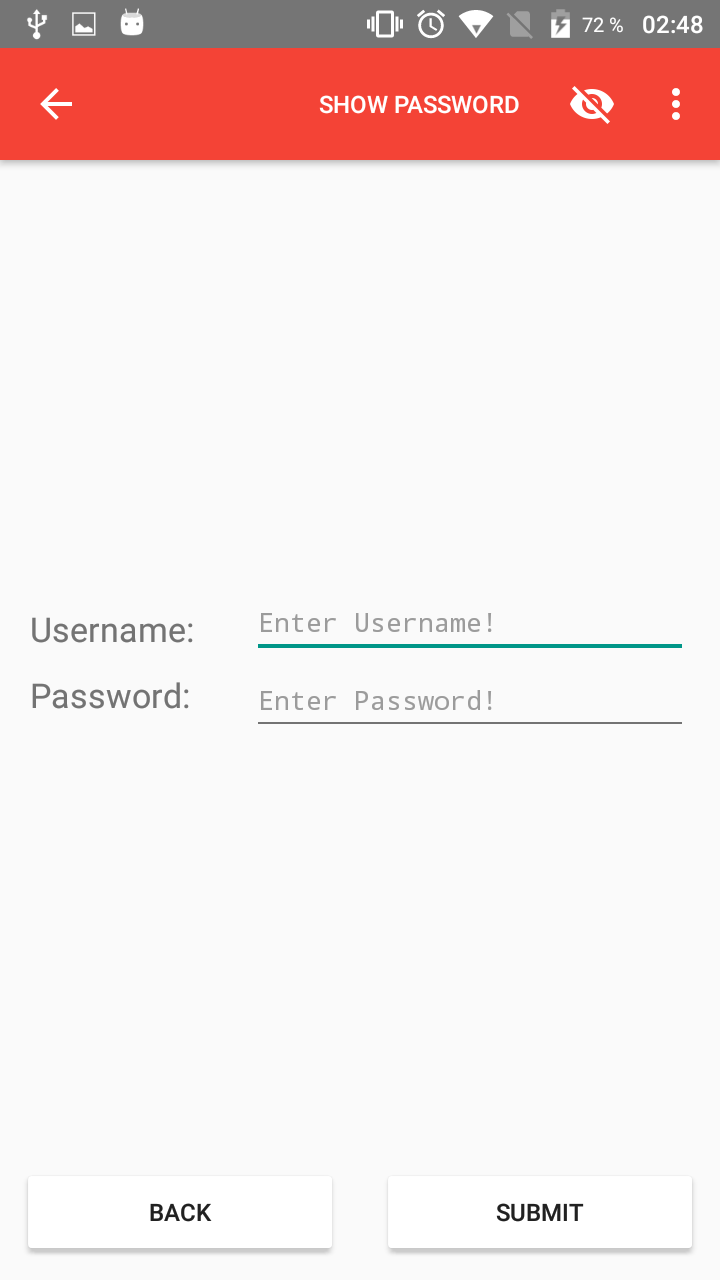
\includegraphics[width=.3\textwidth]{images/stm32kb-loginscreen.png}
		\end{subfigure}
		\begin{subfigure}
			\centering
			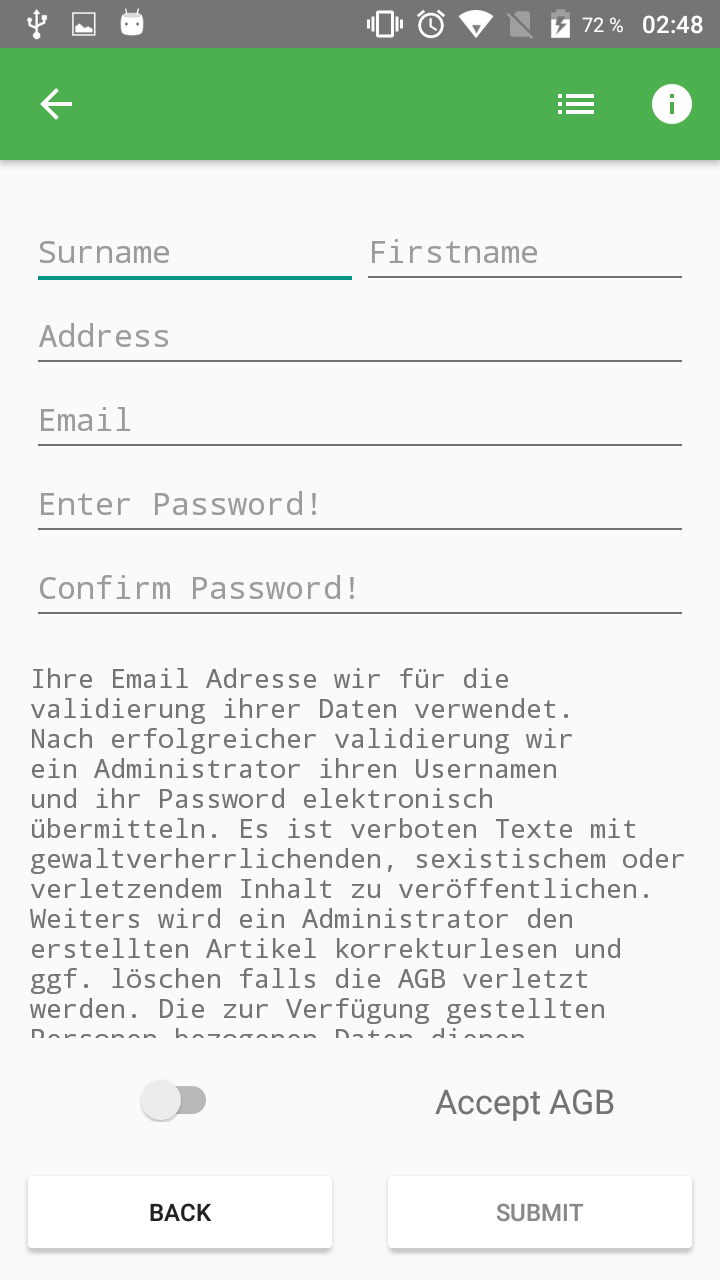
\includegraphics[width=.3\textwidth]{images/stm32kb-registerscreen.png}
		\end{subfigure}
		\begin{subfigure}
			\centering
			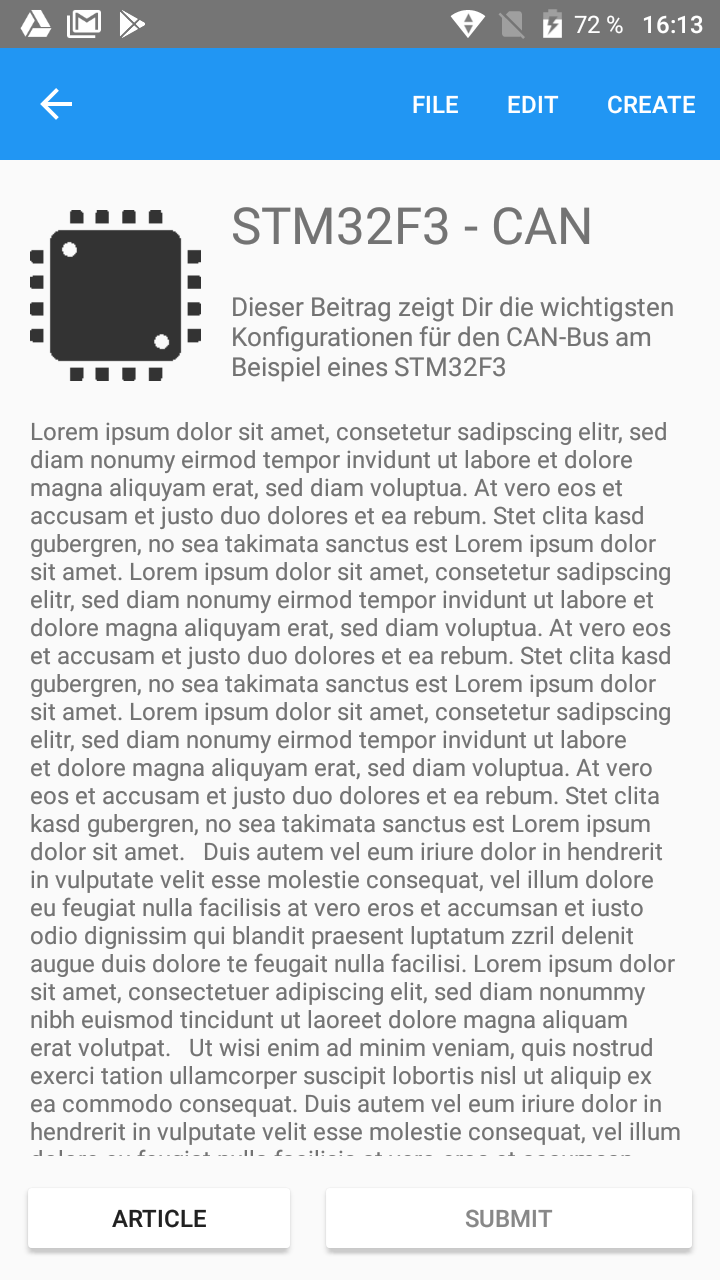
\includegraphics[width=.3\textwidth]{images/stm32kb-articlescreen.png}
		\end{subfigure}
		\caption{Design der STM32KB App - v.l.n.r. Login, Register, Lesen}
		\label{fig:stm32kbApp}
	\end{figure}

	Für die Entwicklung beider CP-Apps wurde eine andere Art der Menüführung herangezogen. Statt einer Navigation über Buttons und Pfeile sind die funktionalen Anforderungen in Form von Tabs umgesetzt worden. Ein Tabbed Layout steht sowohl unter Xamarin.Native als auch Xamarin.Forms zur Verfügung und wird von dem jeweiligen Zielbetriebssystem Renderer so gerendert das es dem Typischen Design Merkmalen entspricht.

	\newpage
	In Abbildung \ref{fig:stm32cpApp} ist das veränderte Menü durch Tabs ersichtlich. Dem Anwender wird durch ein übersichtlicheres Design die Handhabung der Applikation vereinfacht.

	\begin{figure}[h!]
		\centering
		\begin{subfigure}
			\centering
			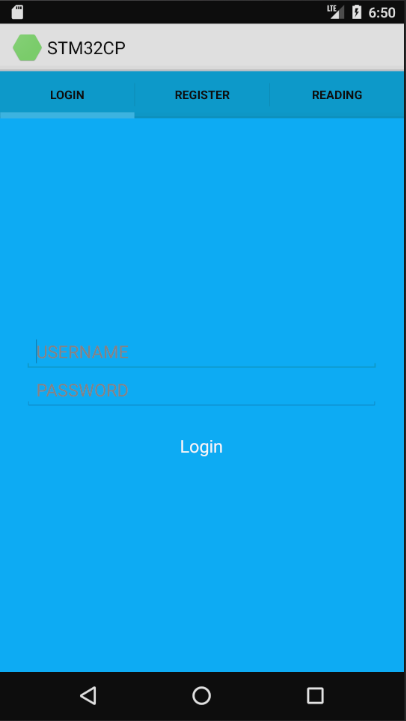
\includegraphics[width=.3\textwidth]{images/STM32CP_Droid-final.png}
		\end{subfigure}
		\begin{subfigure}
			\centering
			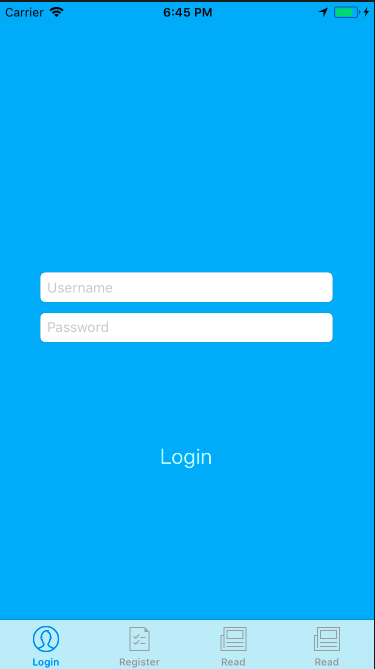
\includegraphics[width=.3\textwidth]{images/STM32CP_iOS-final.png}
		\end{subfigure}
		\caption{Design der STM32CP App}
		\label{fig:stm32cpApp}
	\end{figure}

	Da die STM32CP Applikation mit Xamarin.Native entworfen wurde, musste das Design sowohl für Android s.h. Abbildung \ref{fig:stm32cpApp} links als auch iOS, rechts in Abbildung \ref{fig:stm32cpApp}, getrennt entworfen werden. Zwar klingt dies nun nach doppelten Aufwand für das Design, jedoch hielt sich dies in Grenzen. Das Design einer iOS App ist durch das \textit{Storyboard}, welches für iOS Apps verwendet wird, rasch entworfen. Per Drag\&Drop lassen sich die gewünschten UI Elemente im Layout platzieren und müssen durch Anpassung der \textit{Constraints}\footnote{Durch einen Constraint wird eine Beziehung zwischen Rahmen des Layouts und dem UI Element erzwungen, damit dessen relative Position immer gleich ist} positioniert werden. Für das Design der Android Version kann auch die \textit{XML} Dateien der STM32KB App zurückgegriffen werden sodass mit Copy\&Paste bestimmter Elemente das Design rasch entworfen ist.

	Auf Basis der Erfahrungen die, während der Spezifizierung als auch der Programmierung der CP Variante einer Nativen Android Applikation, gesammelt wurden sollen diese dabei helfen die MCKB App mit Xamarin.Forms zu entwickeln.
	\newpage

\section{Applikations Spezifizierung}
\label{sec:mckspecs}

	Die Spezifizierungen sollen weitestgehend an die vorhergehenden Applikationen anknüpfen. Ein Schlüsselwort wie muss, erzwingt die Umsetzung während sollte, die Möglichkeit der Umsetzung vorschlägt.

	Die Spezifizierungen umfassen folgende Bereiche:
	\begin{itemize}
		\setlength\itemsep{0em}
		\item Design
		\item Funktionale Anforderungen
		\item Nicht Funktionale Anforderungen
	\end{itemize}

	\textbf{Design:} Das Design der App muss mit maximal drei Menüebenen bedienbar sein. Sofern Xamarin.Forms ein Tabbed Layout zur Verfügung stellt so sollte dieses für eine bestmögliche Benutzerfreundlichkeit verwendet werden. Für die Auflistung der Artikel ist folgende Hierarchie zu wählen:
	\begin{itemize}
		\setlength\itemsep{0em}
		\item Dropdown für Kategorien
		\begin{itemize}
			\setlength\itemsep{0em}
			\item Kategorie 1 - i.e. \textbf{STM32F1}
			\begin{itemize}
				\setlength\itemsep{0em}
				\item Unterkategorie 1.1 - i.e. \textbf{STM32F1 - UART}
				\item Unterkategorie 1.2 - i.e. \textbf{STM32F1 - CAN}
			\end{itemize}
		\end{itemize}
	\end{itemize}
	Bezüglich der Farbwahl sollte diese harmonisch sein, demnach blasse Farben die nicht zu sehr in den Vordergrund drängen.

	\textbf{Funktionale Anforderungen }sollen jene Funktionalitäten beschreiben die direkt mit den Anforderungen an die Applikation zusammen hängen. Funktionale Anforderungen können nach folgenden Schema\footnote{Das SRS Dokument wurde in der Vorlesung Software Engineering im 4. Semester vorgestellt} definiert werden:
	\begin{table}[h]
		\centering
		\begin{tabular}{ll}
			Use Case                    &  Name der Anforderung\\ \hline
			Kurzbeschreibung            &  Kurze Definition was passieren soll\\ \hline
			Vorbedingung                &  Was muss vorher gegeben sein\\ \hline
			Nachbedingung               &  Wie ist der Zustand nachher\\ \hline
			Fehlersituation             &  Welcher Fehler kann auftreten\\ \hline
			Systemzustand im Fehlerfall &  - \\ \hline
			Akteure                     &  Wer verwendet die Anforderung\\ \hline
			Standardablauf              &  Systematischer Ablauf für die Anforderung\\ \hline
			Alternativabläufe           &  - \\ \hline
			Trigger                     &  Wie wird die Anforderung angestoßen
		\end{tabular}
		\caption{Standard Schema für Funktionale Anforderungen (\textbf{Use Cases}) laut SRS}
		\label{my-label}
	\end{table}

	\newpage Die in Tabelle \ref{tab:autorlogin} dargestellte Anforderung musste nicht angepasst werden.
	\begin{table}[h!]
		\centering
		\begin{tabular}{lp{11cm}}
			\textbf{Use Case}        &  \textbf{Autor Login}\\ \hline
			Kurzbeschreibung &  Anwender können sich als Autoren anmelden\\ \hline
			Standard Ablauf  &  
				\begin{tabular}[c]{@{}l@{}}
					1. Der Anwender öffnet die App\\ 
					2. Der Tab \textbf{Login} wird ausgewählt\\
					3. Der Anwender gibt \textit{Username} und \textit{Password} ein \\
					4. Die Applikation übermittelt die eingegebenen Daten an die\\Datenbank und lässt diese überprüfen. \\
					5. Bei erfolgreicher Prüfung ist der User für die Dauer der Ver-\\wendung der Applikation als Autor angemeldet und kann (so-\\fern die Funktion implementiert ist) Artikel erstellen oder be-\\arbeiten
				\end{tabular}\\ 
		\end{tabular}
		\caption{Autoren Login - Funktionale Beschreibung}
		\label{tab:autorlogin}
	\end{table}

	Die in Tabelle \ref{tab:autorregister} beschriebene Anforderung wurde in der Ersten CP Version angepasst. In der Nativen Version der Applikation wurden nach Eingabe der Daten vier Fragen an den Anwender gestellt um dessen Wissen über Mikrocontroller zu prüfen. Die Ergebnisse der Fragen und die Daten aus dem Registrierungsformular wurden anschließend an einen Administrator der App übermittelt, damit dieser den neuen Benutzer freischalten kann. Der Schritt mit den Fragen zur Wissensüberprüfung wurde nicht implementiert um nur essentielle Funktionale Anforderungen zur Verfügung zu stellen.
	\begin{table}[h!]
		\centering
		\begin{tabular}{lp{11cm}}
			\textbf{Use Case}        &  \textbf{Autor registrieren}\\ \hline
			Kurzbeschreibung &  Anwender können sich registrieren um als Autoren freigeschaltet zu werden \\ \hline
			Standard Ablauf  &  
				\begin{tabular}[c]{@{}l@{}}
					1. Der Anwender öffnet die App\\ 
					2. Der Tab \textbf{Registrieren} wird ausgewählt\\
					3. Der Anwender befüllt alle Eingabefelder \\
					4. Der Anwender muss den Hinweis auf Freischaltung durch einen\\ Administrator zustimmen \\
					5. Dem Benutzer wird visuell mitgeteilt das eine Registrierungs-\\anfrage gestellt wurde
				\end{tabular}\\ 
		\end{tabular}
		\caption{Autor registrieren - Funktionale Beschreibung}
		\label{tab:autorregister}
	\end{table}

	\newpage Als letzte Funktionale Anforderung ist in Tabelle \ref{tab:artikelread} die Anforderung an das Lesen von Artikeln beschrieben. Diese Anforderung ist ein Zentraler Baustein für die Implementierung des gemeinsamen Codes für die Geschäftslogik.
	\begin{table}[h!]
		\centering
		\begin{tabular}{lp{11cm}}
			\textbf{Use Case}        &  \textbf{Artikel lesen}\\ \hline
			Kurzbeschreibung &  Benutzer können Artikel lesen \\ \hline
			Standard Ablauf  &  
				\begin{tabular}[c]{@{}l@{}}
					1. Der Anwender öffnet die App\\ 
					2. Der Tab \textbf{Lesen} wird ausgewählt\\
					3. Sofern neue Artikel zur Verfügung stehen können diese\\durch Bestätigung eines Hinweises herunter geladen werden\\
					4. In der Page erscheint ein Drop Down Menü zur Auswahl\\ der Kategorie \\
					5. Der Anwender wählt eine Kategorie und gelangt in die Un-\\terkategorie\\
					6. Es werden die Artikel der korrespondierenden Kategorie\\dargestellt
				\end{tabular}\\ 
		\end{tabular}
		\caption{Artikel lesen - Funktionale Beschreibung}
		\label{tab:artikelread}
	\end{table}

	\textbf{Nicht funktionale Anforderungen:}

% \subsection{Funktionale Anforderungen}
% \label{sec:mckbfunkcspecs}
	
% \subsection{Nicht Funktionale Anforderungen}
% \label{sec:mckbnonfuncspecs}

\section{Unterschiede zur Xamarin.Native Version}
\label{sec:mckbspecs}














